\chapter{Model training and device classification results}

In the previous chapters we described how to create a Neural Network classifier able to perform the device identification task and how to obtain and preprocess a dataset to train the classifier on. In this chapter we present and discuss the results of the training of the classifier on the two proposed dataset alongside with an evaluation of its performances.

As said before the results presented in this chapter are obtained after dividing the datasets in three subsets: the training set over which the classifier are trained, the validation set, used to monitor the performances during the training and the test set, used to evaluate the real performances of the classifiers.

In section \secref{res_lb} we will discuss the specific architecture selected for each dataset and show how the choice of the lookback value influences the model performances. In \secref{res_test} we will then show the results of the training of the classifier and its final performances. Finally in \secref{res_unseen} we will presents an example of the implementation of said classifier in case of devices not included in the dataset used for training and performance testing.

\section{Classifier architecture and time series length}\label{res_lb}

In \chapref{chap4} we presented the statistic and the class division of the 4SICS and IoT Sentinel dataset, respectively in \tabref{tab:4sicsdataset} and \tabref{tab:iotdataset}. During the preprocessing operation the 4SICS dataset timeseries were created using a value of the lookback, defined in \secref{fig:ts_processing}, of $L=100$. The IoT dataset on the other hand was preprocessed using a value $L=30$. As previously stated the choice of using a smaller lookback value is made in order to maximize the number of timeseries, and consequently the dataset dimension, with the goal of maximizing the final performance of the model. 

This choice however is not compatible with the use of the 1B\_AP architecture, namely the general proposed model, so the 1B\_NP architecture should be used instead. The value $L=30$ in particular correspond to the estimation of the possible lookback lower bound. This estimation was done by training a classifier created using the 1B\_NP architecture and different values of the lookback $L$. The dataset used for this estimation in the 4SICS dataset due the higher number of time series that are contained in it. 

In \figref{fig:res_lb_val} the value of the model accuracy over the training and validation dataset is shown, with respect to the chosen lookback value. As we can see from these plots for using values of $L=10,20$ results in divergence in the training and validation loss function. This behaviour indicates the presence of overfitting during the training. This may be explained considering that, for low $L$ valus some variety is lost in the time series and, consequently, the model is too complex for the provided input dimension.

The classifier trained with $L=30$ on the other hand does not present such behaviour justifying the choice made for the lookback value for this architecture. Additional plots of the loss function and model accuracy for higher values of the lookback are shown in \appref{app:lb_bonus_res}.


\begin{figure}[!h]
    \centering
    \begin{minipage}[c]{0.49\textwidth}
        \vspace{0pt}
        \centering
        \subfloat[Loss function with lookback $L=10$]{
        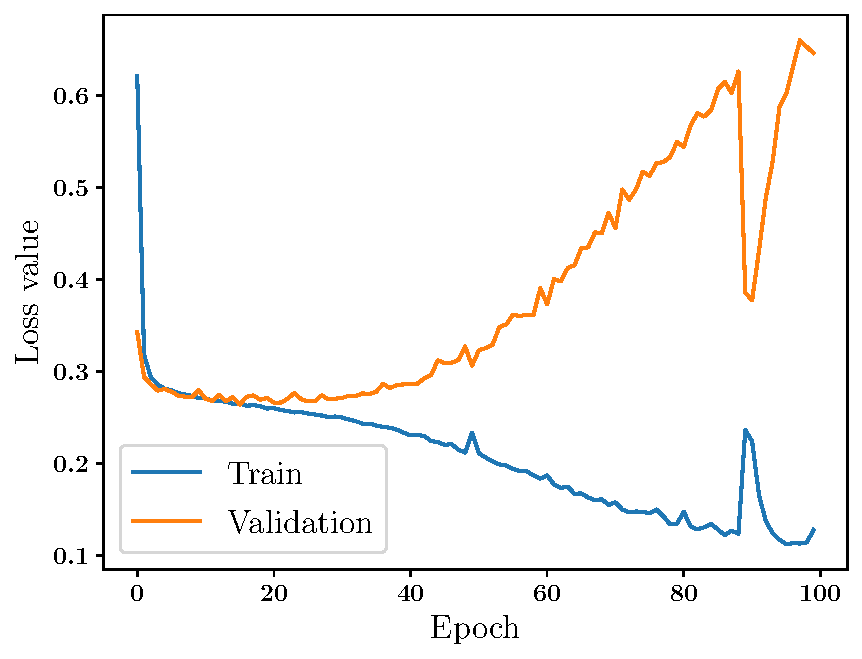
\includegraphics[width=\textwidth]{images/results/LB_test_10_20210613-180735__type_1branch_no_pool__st_scale_sub__lb_10__act_elu__nf_16__ks_10__nn_50__l2_1e-05__bs_200__ep_100__loss.pdf}
            \label{fig:lb_10_loss}
        }
    \end{minipage}%
    \hfill%
    \begin{minipage}[c]{0.49\textwidth}
        \vspace{0pt}
        \centering
        \subfloat[Accuracy with lookback $L=10$]{
        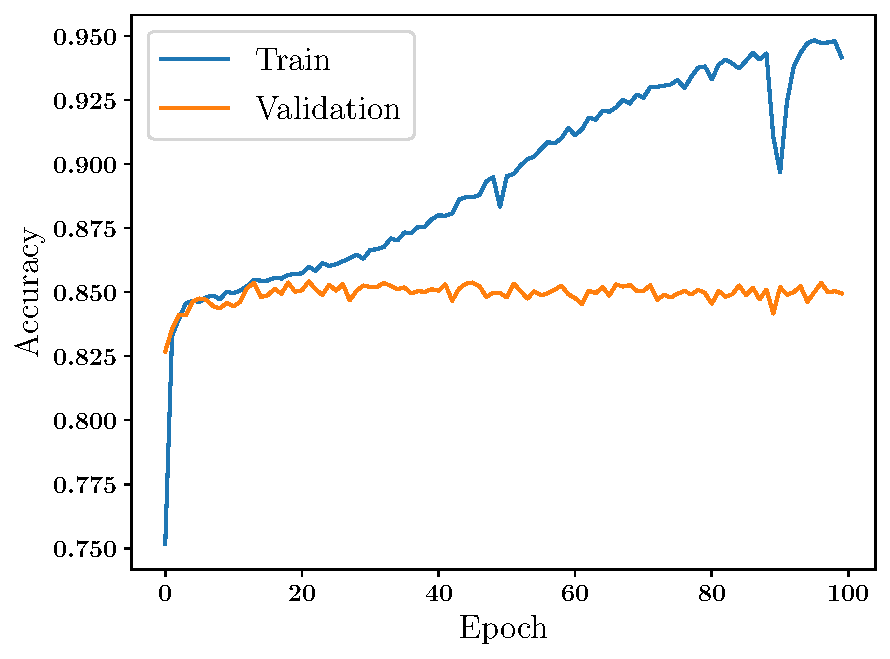
\includegraphics[width=\textwidth]{images/results/LB_test_10_20210613-180735__type_1branch_no_pool__st_scale_sub__lb_10__act_elu__nf_16__ks_10__nn_50__l2_1e-05__bs_200__ep_100___accuracy.pdf}
            \label{fig:lb_10_acc}
        }
    \end{minipage}
        \begin{minipage}[c]{0.49\textwidth}
        \vspace{0pt}
        \centering
        \subfloat[Loss function with lookback $L=20$]{
        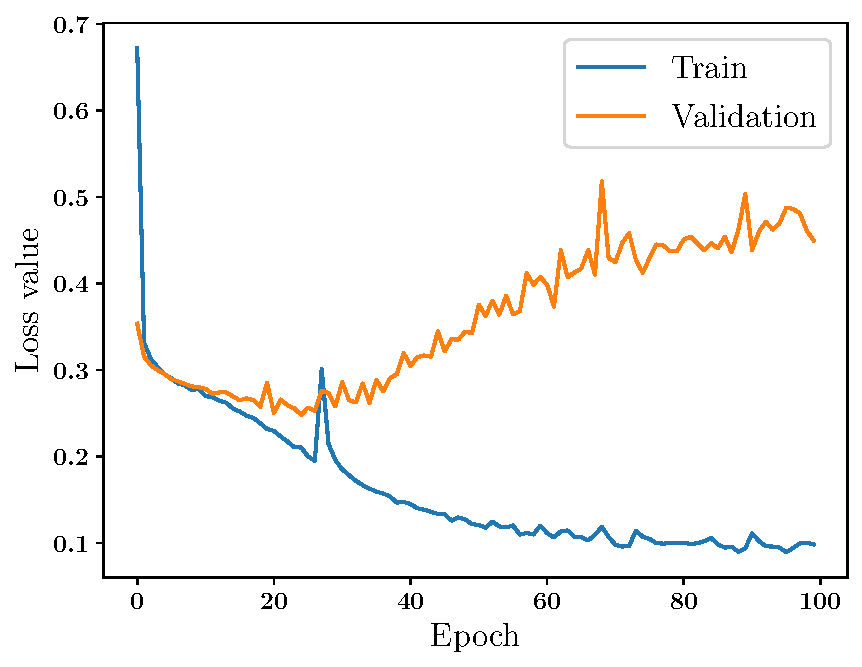
\includegraphics[width=\textwidth]{images/results/LB_test_20_20210613-180946__type_1branch_no_pool__st_scale_sub__lb_20__act_elu__nf_16__ks_10__nn_50__l2_1e-05__bs_200__ep_100__loss.pdf}
            \label{fig:lb_20_loss}
        }
    \end{minipage}%
    \hfill%
    \begin{minipage}[c]{0.49\textwidth}
        \vspace{0pt}
        \centering
        \subfloat[Accuracy with lookback $L=20$]{
        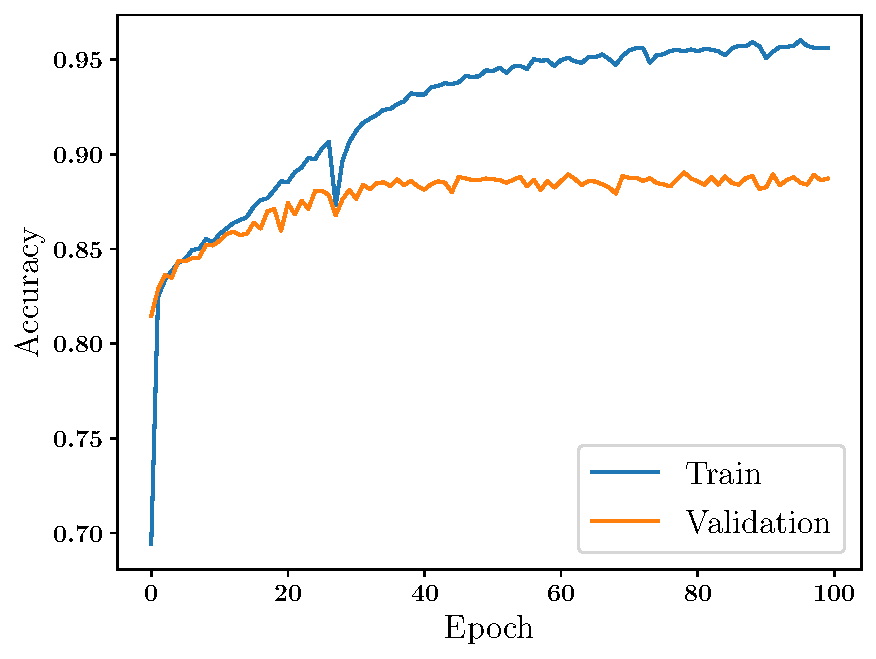
\includegraphics[width=\textwidth]{images/results/LB_test_20_20210613-180946__type_1branch_no_pool__st_scale_sub__lb_20__act_elu__nf_16__ks_10__nn_50__l2_1e-05__bs_200__ep_100___accuracy.pdf}
            \label{fig:lb_20_acc}
        }
    \end{minipage}    \begin{minipage}[c]{0.49\textwidth}
        \vspace{0pt}
        \centering
        \subfloat[Loss function with lookback $L=30$]{
        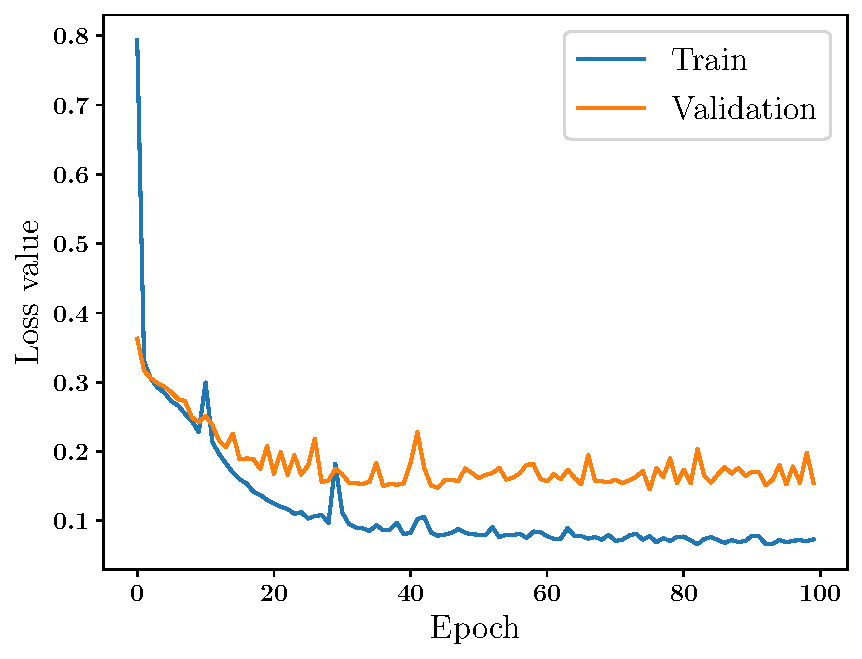
\includegraphics[width=\textwidth]{images/results/LB_test_30_20210613-181249__type_1branch_no_pool__st_scale_sub__lb_30__act_elu__nf_16__ks_10__nn_50__l2_1e-05__bs_200__ep_100__loss.pdf}
            \label{fig:lb_30_loss}
        }
    \end{minipage}%
    \hfill%
    \begin{minipage}[c]{0.49\textwidth}
        \vspace{0pt}
        \centering
        \subfloat[Accuracy with lookback $L=30$]{
        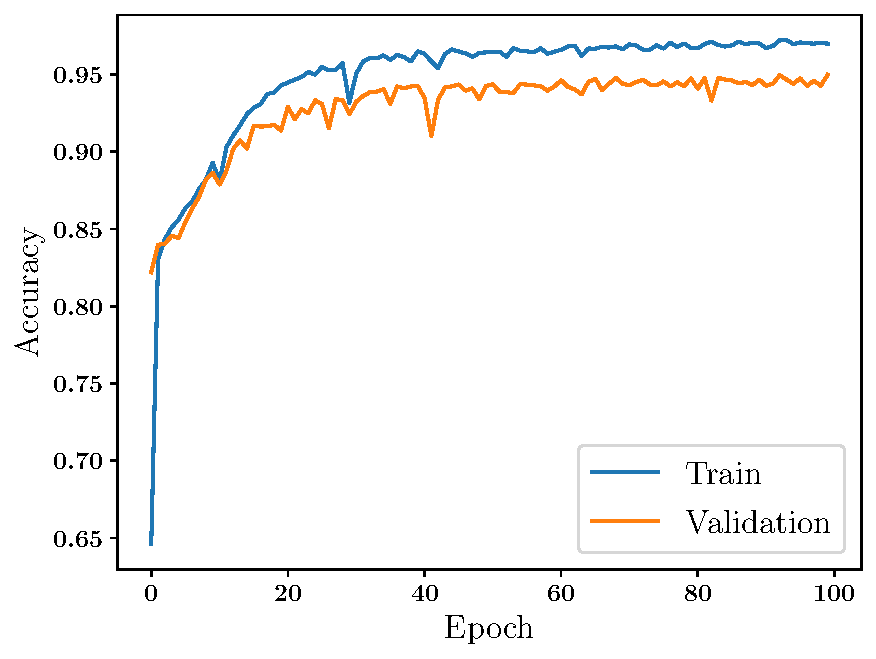
\includegraphics[width=\textwidth]{images/results/LB_test_30_20210613-181249__type_1branch_no_pool__st_scale_sub__lb_30__act_elu__nf_16__ks_10__nn_50__l2_1e-05__bs_200__ep_100___accuracy.pdf}
            \label{fig:lb_30_acc}
        }
    \end{minipage}


    \caption{lookback analysis}
    \label{fig:res_lb_val}
\end{figure}





\section{Model training and final performance}\label{res_test}

In this section we present the final performance of the proposed classifier after the training procedure for both datasets. The performances have been evaluated used the test sets and the possible presence of over or under fitting behaviour is monitored, as shown previously, using the validation set. All the computations have been performed on a machine with a Ryzen 6 core CPU, an NVIDIA GTX 1660 Super GPU and 32GB of memory.




\subsection{4SICS dataset}

As stated previously the chosen architecture for the device classification over the 4SICS dataset in the 1B\_AP model, namely an architecture with one convolutional "branch" with average pooling layers. The selected device classes, shown in \tabref{tab:4sicsdev}, have been preprocessed using a lookback $L=100$. The training was performed for 300 epochs using a batch size \footnote{The batch size indicated after how many samples the free parameters of the Neural Networks should be updated using the backpropagation algorithm} of 200. 

In \figref{fig:4sics_results} the evolution of the loss function and of the model accuracy over the training and validation set are shown. As we can see the model is able to reach high performances and does not show overfitting behaviour. 


\begin{figure}[h]
    \centering
    \begin{minipage}[c]{0.49\linewidth}
        \vspace{0pt}
        \centering
        \subfloat[Loss function during training]{
        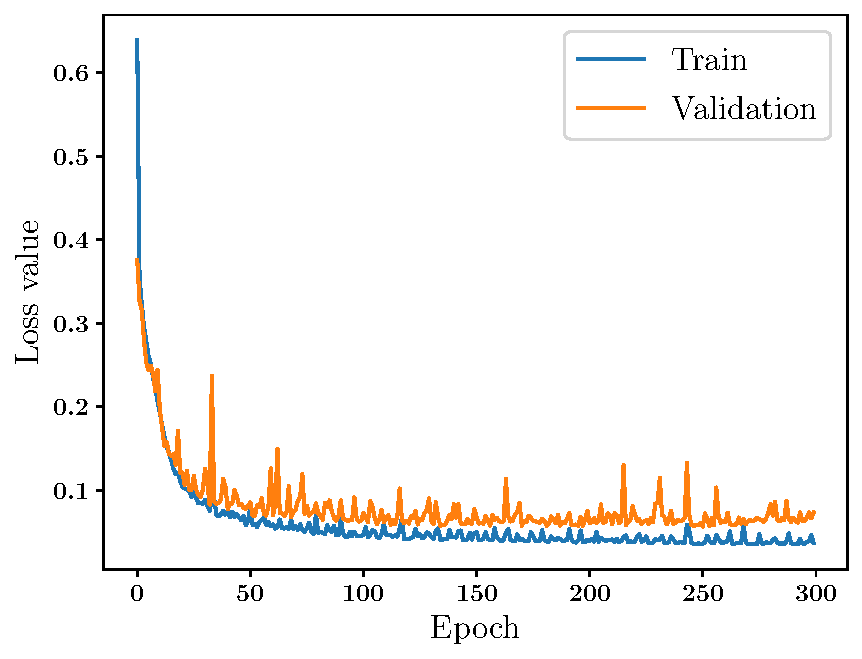
\includegraphics[width=\textwidth]{images/results/4SICS_clasf_20210613-174409__type_1branch__st_scale_sub__lb_100__act_elu__nf_16__ks_10__nn_50__l2_1e-05__bs_200__ep_300__loss.pdf}
            \label{fig:4sics_loss}
        }
    \end{minipage}%
    \hfill%
    \begin{minipage}[c]{0.49\linewidth}
        \vspace{0pt}
        \centering
        \subfloat[Accuracy during training]{  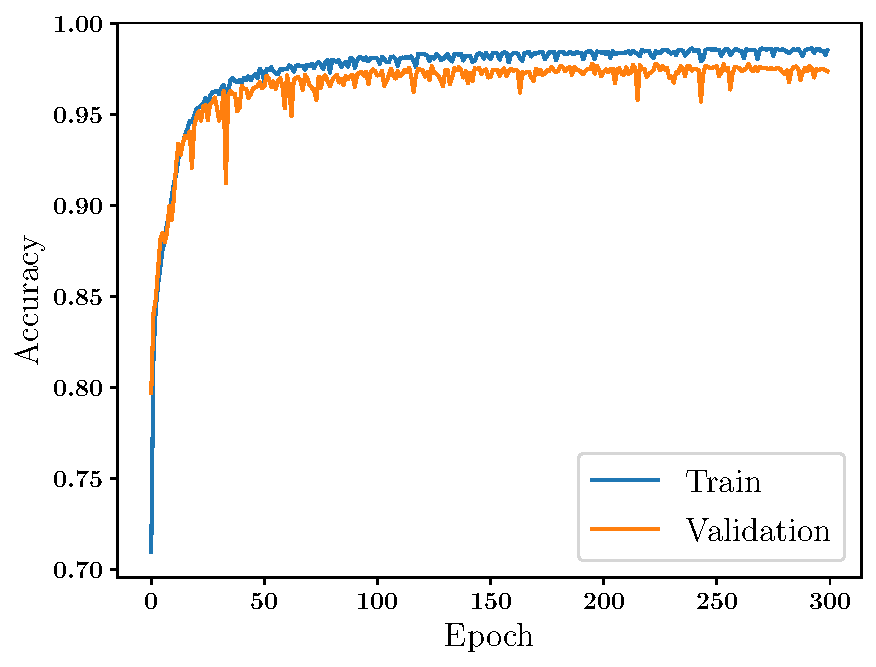
\includegraphics[width=\textwidth]{images/results/4SICS_clasf_20210613-174409__type_1branch__st_scale_sub__lb_100__act_elu__nf_16__ks_10__nn_50__l2_1e-05__bs_200__ep_300___accuracy.pdf}
        \label{fig:4sics_loss}
        }
    \end{minipage}%
    \caption{confronto}
    \label{fig:4sics_results}
\end{figure}

The model performances are evaluated over the test dataset comparing the predicted class of the devices with their true class. This comparison is done using a confusion matrix, shown in \figref{fig:4sics_results_cm}. As we can see for all classes more than 90\% of the predicted labels are correct with the Switch and Router class having 100\% correct predictions. From this matrix we also estimate a 96.2\% overall test accuracy.

\begin{figure}[h]
    \centering
        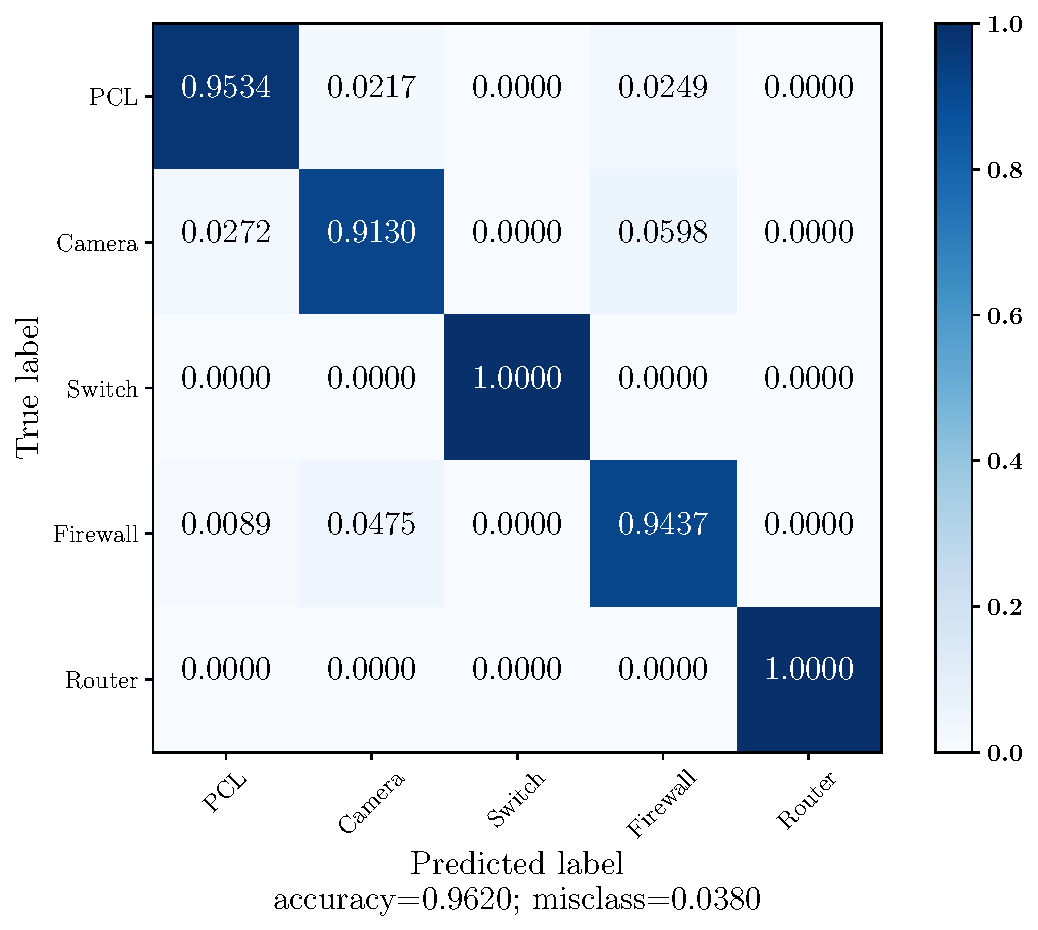
\includegraphics[width=0.6\textwidth]{images/results/4SICS_clasf_20210613-174409__type_1branch__st_scale_sub__lb_100__act_elu__nf_16__ks_10__nn_50__l2_1e-05__bs_200__ep_300___cm.pdf}
    \caption{confronto}
    \label{fig:4sics_results_cm}
\end{figure}

\subsection{IoT dataset}

As stated previously due to the small length of the timeseries the chosen architecture for the device classification over the IoT Sentinel dataset in the 1B\_NP model, namely an architecture with one convolutional "branch" without pooling layers. The selected device classes, shown in \tabref{tab:iotdev}, have been preprocessed using a lookback $L=30$. The training was performed for 300 epochs using a batch size of 100. 

In \figref{fig:iot_results} the evolution of the loss function and of the model accuracy over the training and validation set are shown. As for the previous dataset the model is able to reach high performances and does not show overfitting behaviour, validating the choice of architecture and lookback value. 


\begin{figure}[h]
    \centering
    \begin{minipage}[c]{0.49\linewidth}
        \vspace{0pt}
        \centering
        \subfloat[Loss function during training]{
        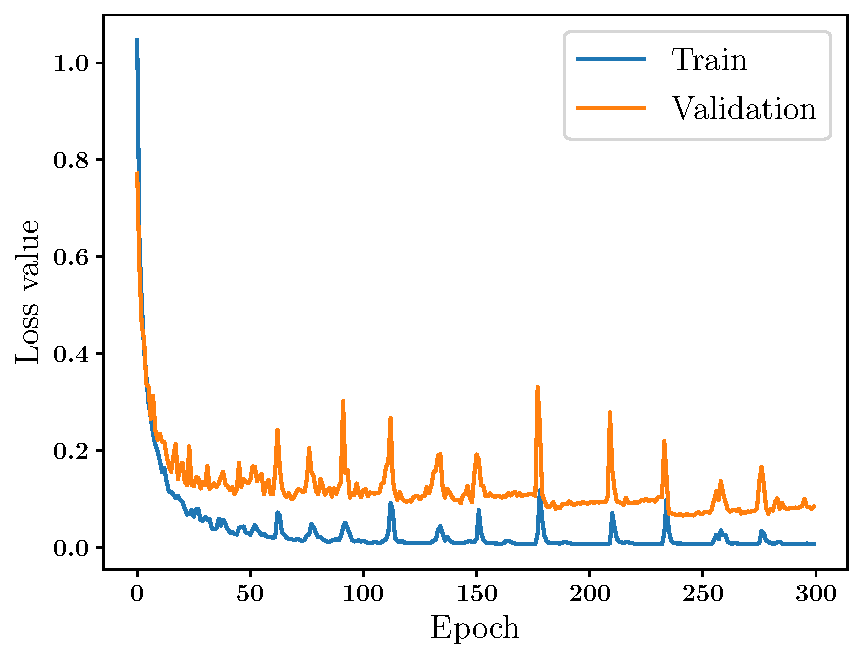
\includegraphics[width=\textwidth]{images/results/IoT_clasf_20210613-175027__type_1branch_no_pool__st_scale_sub__lb_30__act_elu__nf_16__ks_10__nn_50__l2_1e-05__bs_200__ep_300__loss.pdf}
            \label{fig:iot_loss}
        }
    \end{minipage}%
    \hfill%
    \begin{minipage}[c]{0.49\linewidth}
        \vspace{0pt}
        \centering
        \subfloat[Accuracy during training]{  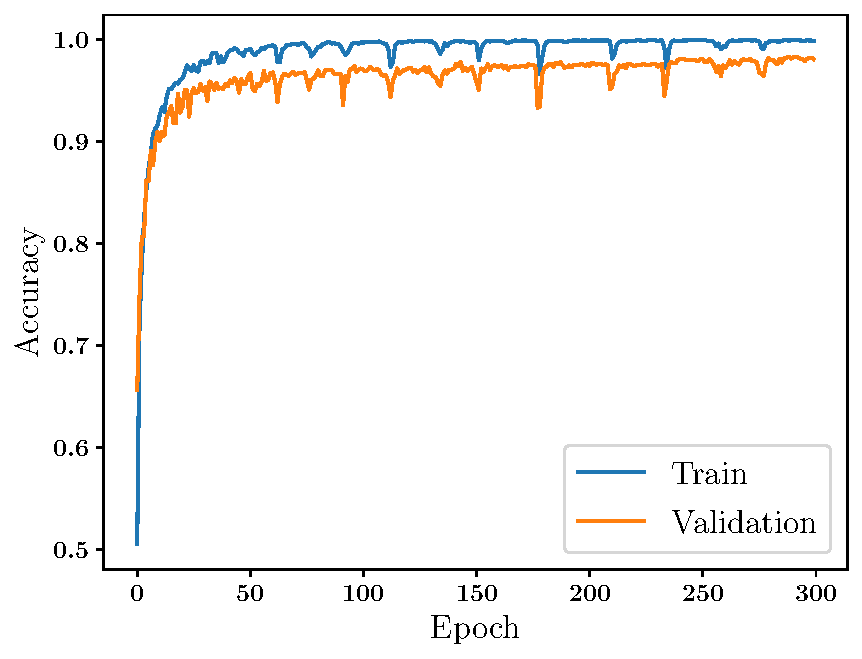
\includegraphics[width=\textwidth]{images/results/IoT_clasf_20210613-175027__type_1branch_no_pool__st_scale_sub__lb_30__act_elu__nf_16__ks_10__nn_50__l2_1e-05__bs_200__ep_300___accuracy.pdf}
        \label{fig:iot_loss}
        }
    \end{minipage}%
    \caption{confronto}
    \label{fig:iot_results}
\end{figure}


As for the previous model we evaluate the model performances using a confusion matrix, shown in \figref{fig:4sics_results_cm}. For this dataset the classifier is able to reach a test accuracy higher than 95\% for all the classes with an overall accurcay of 98.6\%

\begin{figure}[h]
    \centering
        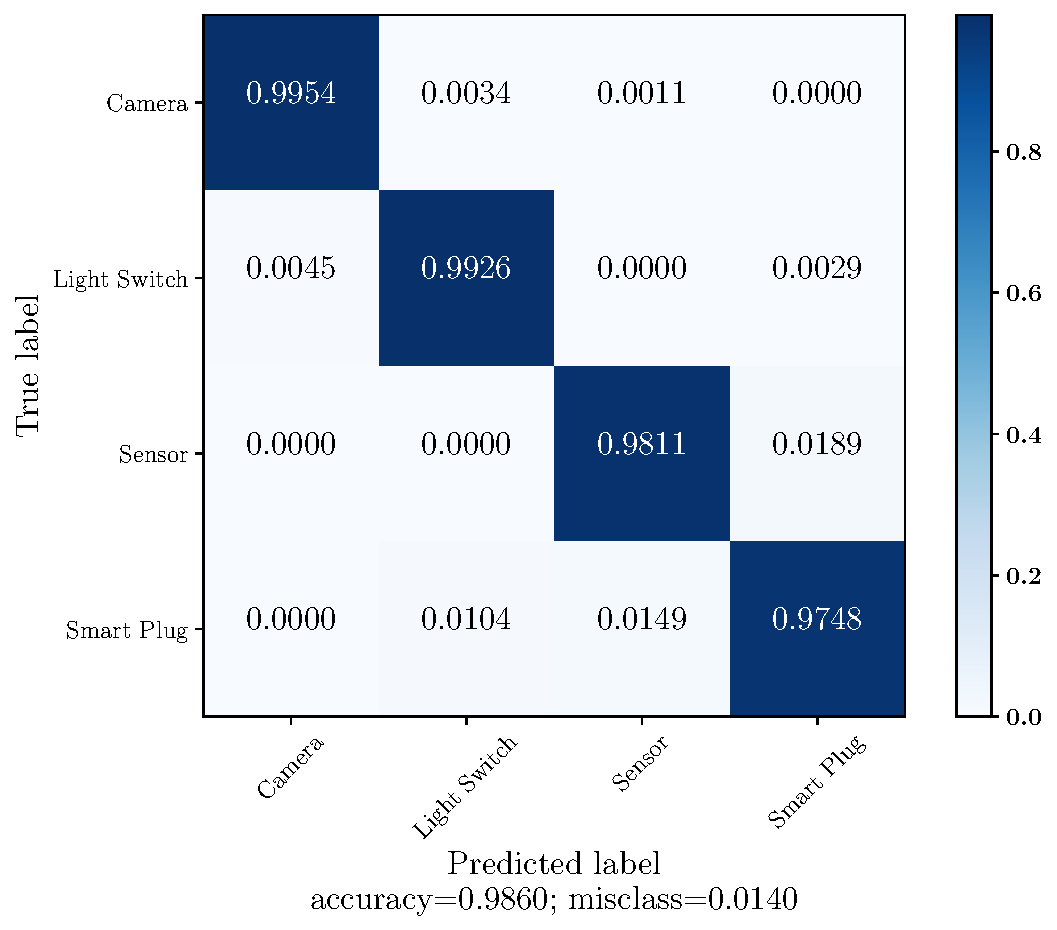
\includegraphics[width=0.6\textwidth]{images/results/IoT_clasf_20210613-175027__type_1branch_no_pool__st_scale_sub__lb_30__act_elu__nf_16__ks_10__nn_50__l2_1e-05__bs_200__ep_300___cm.pdf}
    \caption{confronto}
    \label{fig:iot_results_cm}
\end{figure}



\section{"Unseen" device classification}\label{res_unseen}

In the previous section we show that the proposed model is able, with great accurcay, of correctly of performing the identification of a device.



\section{Discussion}

Looking at the results obtained for both datasets we can draw some conclusion. The first important thing to highlight is the very high test accuracy obtained in both cases 
